% \begin{figure}[t]
%     \centering
%     \includegraphics[width=\linewidth]{figure/entropy_histogram.pdf}
%     \caption{placeholder: student}
%     \label{fig:opd_entropy}
% \end{figure}

% \section{Improving On-Policy Distillation}
%\section{Motivating Investigation on OPD}
% \yj{maybe push to right?}
\section{Diversity Degradation and Instability in On-Policy Distillation} \label{sec:limit_opd}

In \S\ref{sec:diversity}, we first analyze token-level entropy distributions to identify diversity degradation after on-policy distillation due to reverse KL. We then show that reverse KL produces unstable learning signals when teacher entropy is high, with the student's top-k predictions failing to converge in \S\ref{sec:instability}.
% We also demonstrate that reverse KL leads to unstable learning on high-entropy tokens, limiting the student's ability to capture the teacher's uncertainty (\S\ref{sec:instability}).
%We then provide a deeper understanding through a controlled experiment, demonstrating that this degradation is correlated with the student's failure to learn from high-entropy tokens of the teacher model (\S\ref{sec:instability}). 

%%%% Prev version
% % maybe different name? Analyzing On-Policy Distillation
% In this section, we first analyze the problem of diversity degradation after on-policy distillation (\S\ref{sec:diversity}). 
% % We then demonstrate that this is related to high-entropy tokens of the teacher model not being learned by the student model in a simple toy experiment (\S\ref{sec:instability}). 
% We then demonstrate, through a simple toy experiment, that diversity degradation is correlated to the student’s failure to learn from high-entropy tokens of the teacher model (\S\ref{sec:instability}).
% % Based on these observations, we propose a distillation approach that adaptively adjusts the training objective according to the teacher’s uncertainty (\S\ref{sec:main_method}).

\subsection{Token-Level Entropy Analysis}\label{sec:diversity}

% new version
In domains that require complex reasoning, such as mathematical and multi-step reasoning tasks, high-entropy tokens\footnote{We use {\em high-entropy token} as shorthand for a token at a position where the teacher's conditional distribution has high entropy.} in the teacher model are not merely noise but encode important knowledge in the form of multiple plausible reasoning paths and meaningful uncertainty~\cite{wang2025beyond, cheng2025reasoning}. However, on-policy distillation may fail to properly capture this knowledge. As discussed in \S\ref{sec:pre_opd}, it typically minimizes the reverse KL divergence, a mode-seeking objective that favors fast convergence at the cost of reduced exploration, thereby hindering the transfer of the teacher's uncertainty to the student.
%However, on-policy distillation typically minimizes the reverse KL divergence, which exhibits a mode-seeking property that reduces exploration and enables fast convergence. While this behavior is beneficial for efficiency, it can hinder the transfer of uncertainty from the teacher to the student.

% To examine this effect, we generate responses from both the teacher model and the fine-tuned student model trained via on-policy distillation on the AIME24 and AIME25 benchmarks, and analyze their token-level entropy. 

To examine this effect, we generate responses from the teacher model (Qwen3-8B~\cite{yang2025qwen3}) and an on-policy-distilled student (Qwen3-1.7B-Base) and evaluate on AIME24 and AIME25 prompts~\cite{maa_aime}, and analyze their token entropy distributions (see \S\ref{sec:experimental_settings} for more details on the experimental setup).
% \autoref{fig:opd_entropy} presents the entropy distribution of the student and teacher model. 
We find that the distilled student retains fewer high-entropy tokens (entropy $\geq 1.0$) than the teacher, specifically only 6.8\% compared to 18.5\% of the teacher (see \autoref{fig:entropy_histogram} in \S\ref{sec:token_level_entropy} for full histogram).
% As shown in \autoref{fig:opd_entropy}, the distilled student retains fewer high-entropy tokens than the teacher.
This suggests that reverse KL drives aggressive mode-seeking behavior rather than preserving the teacher's inherent uncertainty. 
% The comparison reveals a degradation in diversity in the student model after training, reflected in a reduction in token-level entropy. 
% It retains fewer high-entropy tokens than the teacher, suggesting that on-policy distillation with reverse KL drives aggressive mode-seeking behavior rather than preserving the teacher's inherent uncertainty.
% Specifically, the fine-tuned student model retains fewer high-entropy tokens compared to the teacher model, indicating that on-policy distillation with reverse KL fails to transfer the uncertainty encoded in the teacher and instead encourages strongly mode-seeking behavior. 
% We investigate this phenomenon further by analyzing the impact of teacher uncertainty when optimizing the reverse KL objective in a simplified setup.
%In the following section, we investigate this phenomenon further through a controlled experiment.

% old version
% On-policy distillation that minimizes the reverse KL divergence exhibits a mode-seeking property, reducing unnecessary exploration and enabling fast convergence. However, we observe a diversity degradation (i.e., decrease of token-level entropy) in the student model after training. Specifically, using both the teacher and the fine-tuned student model (via on policy distillation), we generate responses on the AIME 2024 and 2025 benchmarks and analyze the token-level entropy of the generated outputs. As shown in \autoref{fig:entropy_student} and \autoref{fig:entropy_teacher}, we find that the fine-tuned student model retains less high-entropy tokens compared to the teacher model. In domains that require complex reasoning, such as reasoning tasks, high entropy tokens in the teacher are not merely noise but encode important knowledge in the form of multiple reasoning paths or meaningful uncertainty. However, on policy distillation fails to transfer this uncertainty encoded in the teacher model to the student model, as they exhibit strong mode-seeking behavior. We investigate this further by analyzing the impact of teacher uncertainty during optimizing reverse KL in a simplified setup.


% By concentrating probability mass on a narrower subset of tokens, reverse KL reduces the effective diversity of the student distribution, limiting exploration during on-policy training.
% These observations also indicate that for tokens where the teacher exhibits high entropy, the teacher's diversity is not adequately transferred to the student during on-policy distillation. Next, we investigate why this happens by analyzing the impact of teacher uncertainty during optimizing reverse KL in a simple toy setup.
\begin{figure}[t]
    \centering
    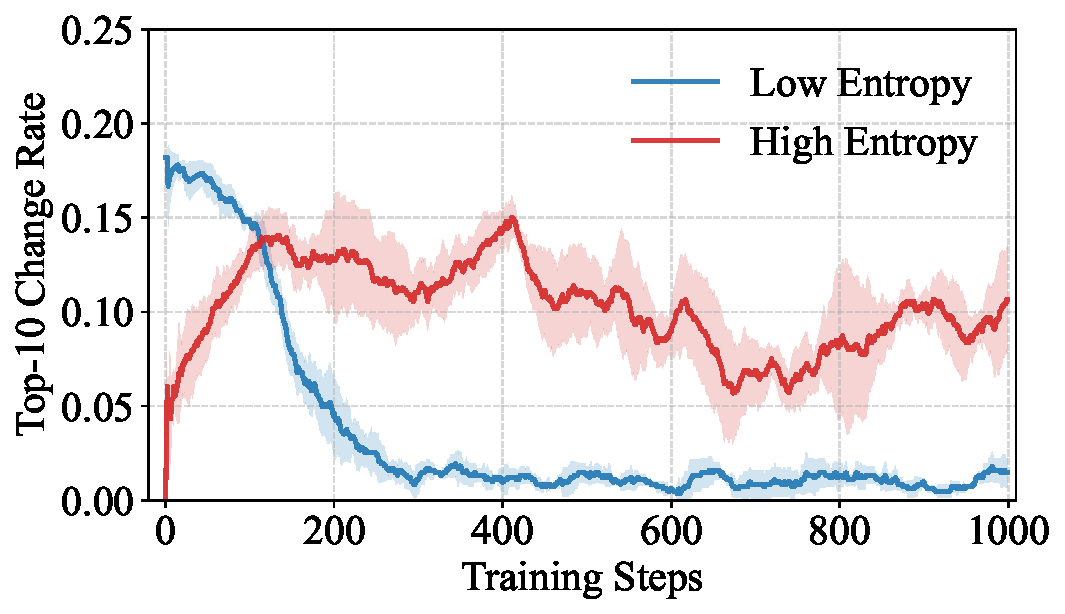
\includegraphics[width=0.9\linewidth]{figure/entropy_stability_comparison.pdf}
    \caption{Top-10 change rate for Scenario A (blue), where the teacher distribution has low entropy, and Scenario B (red), where the teacher distribution has high entropy across 3 seeds. For Scenario B, a student optimized with reverse KL fails to capture the teacher’s distribution, as evidenced by %frequent Top-1 token changes and highly 
    persistently high and fluctuating Top-10 change rates.}
    \label{fig:topk_change}
    \vspace{-5pt}
\end{figure}

\begin{table}[h]
\centering
\small
%\vspace{0.2cm}
\caption{Top-1 Change Count for low teacher entropy scenario and a high teacher entropy scenario. We observe that when the teacher entropy is high, the top-1 index frequently changes.}
\begin{tabular}{ccc}
    \toprule
    \textbf{Teacher Entropy} & \textbf{Temp.} & \textbf{Top-1 Change Count} \\
    \midrule
    (A) Low     &  0.3 & $7.3\pm1.6$ \\
    (B) High    &  1.0 & $84.0\pm16.7$ \\
    \bottomrule
\end{tabular}
\label{tab:top1_change}
\end{table}

\subsection{Instability of Reverse KL-based Reward}\label{sec:instability}


% Through a toy experiment, we analyze how reverse-KL-based reward optimization behaves under different levels of teacher uncertainty.
To gain insight, we first conduct a simplified toy experiment to analyze how reverse KL-based reward optimization behaves under different levels of teacher uncertainty.

\textbf{Toy setup.} We study how a student learns from a teacher via reverse KL policy gradients, in a setting that retains the essential characteristics of having a teacher distribution with multiple modes and a student with limited coverage. To simplify matters, we remove the autoregressive conditioning on context $\mathbf{c}_t$. This reduces the distributions to categorical distributions over $V$ indices (here $V = 80$) and no longer requires complex LLMs.

The teacher distribution $P_{\tt te}$ is constructed as follows. We sample logits $\mathbf{z}\in\mathbb{R}^V$ i.i.d.\ from $\mathcal{N}(0,1)$, then overwrite five randomly chosen entries with larger values $\{1.7, 1.9, 2.1, 2.3, 2.5\}$ to create five modes. We then apply temperature scaling: 
\[
P_{\tt te}(x)=\mathrm{softmax}(\mathbf{z}/T)_x.
\]
We consider two scenarios: (A) $T=0.3$, yielding a low-entropy (peaked) teacher, and (B) $T=1.0$, yielding a high-entropy (diverse) teacher. The teacher is fixed throughout training (see \autoref{app:toy_experiment} for a detailed summary and visualization of the distribution).

The student distribution $P_S$ is parameterized by learnable logits $\mathbf{s}\in\mathbb{R}^V$ initialized i.i.d. from $\mathcal{N}(0,1)$. To mimic limited model capacity, we restrict sampling to the student's top-10 indices.
%\footnote{This setup mirrors top-$k$ logit matching commonly used in LLM distillation, where only the $k$ highest-probability tokens are considered during training.} 
We denote this capacity-limited (top-10) student distribution as $P_{S^{10}}$.

\textbf{Optimization.} At each step, we sample an index $x\sim P_{S^{10}}$ and compute the reward 
\[
r(x) = \log P_{\tt{te}}(x) - \log P_{S^{10}}(x),
\]
corresponding to a sample-based estimate of the negative reverse KL. We then update the sampled logit via $s_x \leftarrow s_x + \eta r(x)$ where $\eta$ denotes the learning rate.

\textbf{Metrics.} We track two metrics during training: (1) {\em the top-10 change rate}, defined as the Jaccard distance~\cite{jaccard1901etude}
$\left(
1 - \frac{|\mathcal{S}_{t} \cap \mathcal{S}_{t-1}|}{|\mathcal{S}_{t} \cup \mathcal{S}_{t-1}|}
\right)$ between the sets of top-10 tokens $\mathcal{S}_{t-1}$, $\mathcal{S}_{t}$ at steps $t-1$ and $t$; and 
(2) {\em the top-1 change count}, the number of times the student's most probable index changes between updates.

\textbf{Results.} As shown in \autoref{fig:topk_change} and \autoref{tab:top1_change}, under the low-entropy teacher (Scenario A), the top-10 change rate decreases steadily and top-1 changes are rare. In contrast, under the high-entropy teacher (Scenario B), training exhibits persistent instability: the top-1 index changes frequently and the top-10 set fails to converge. These results demonstrate that reverse-KL rewards provide unstable learning signals when the teacher distribution is uncertain. This motivates training objectives that more directly transmit the teacher's distributional structure to the student.

% %%%%% Prev version

% Additionally, we design a toy experiment to analyze how the reverse KL-based reward optimization affects learning for different levels of uncertainty in the teacher distribution.

% We consider two scenarios: \textit{(1)} Scenario A, in which the teacher distribution is sharply peaked and exhibits low entropy, analogous to clear and unambiguous token positions; and \textit{(2)} Scenario B, in which the teacher distribution is more diverse and exhibits high entropy, reflecting complex and diverse token positions.
% % teacher distribution is drawn from the standard normal distribution. n = 5, is given 2.5 2.3, 2.1, 1.9, 1,7. given at 5 random positions 
% % The specific details on how each scenario is constructed is in Appendix X.
% % We consider two scenarios, one where the teacher has a clear answer with low entropy and another where the teacher is ambiguous with high entropy, and analyze the behavior of the student after being trained by minimizing reverse KL.

% \paragraph{Toy setup and optimization objective.}

% This toy experiment analyzes the learning dynamics induced by the objective used in on-policy distillation. 
% Specifically, we study how reverse-KL policy-gradient optimization behaves when a support-limited student distribution approximates a multi-modal teacher distribution.

% The teacher is a fixed categorical distribution $P_{\tt te}$ over an index set $\{1,\dots,V\}$.
% We construct its logits as follows. 
% We first sample a logit vector $\mathbf{z}\in\mathbb{R}^V$ i.i.d.\ from $\mathcal{N}(0,1)$.
% We then randomly select $n=5$ indices and overwrite their logits with larger values $\{1.7, 1.9, 2.1, 2.3, 2.5\}$ to create pronounced modes.
% Finally, we apply temperature scaling and a softmax:
% \[
% P_{\tt te}(j)=\mathrm{softmax}(\mathbf{z}/T)_j,
% \qquad j\in\{1,\dots,V\},
% \]
% using $T=0.1$ in Scenario~A and $T=1$ in Scenario~B  (lower $T$ yields a lower-entropy teacher).
% The resulting teacher distribution is fixed throughout training (see Appendix~X for a visualization).

% % The teacher is a fixed categorical distribution $P_{\tt te}$ defined over an index set $\{1,\dots,V\}$. Its logit vector is initialized from the standard normal distribution, but with $n=5$ numbers are randomly selected and assigned larger logit values (i.e., 1.7, 1.9, 2.1, 2.3, 2.5) to create peaks. The logits are then scaled by a temperature parameter $T=0.1$ for scenario A and $T=1$ for scenario B and passed through a softmax, giving the final teacher distribution (see Appendix X for a visualization of the distribution). The teacher distribution is fixed throughout training.
% % The parameter $T$ controls the relative differences between logits and therefore the entropy of the resulting distribution with smaller values of $T$ producing more concentrated distributions. 

% % The student is also a categorical distribution $P_S$ defined over the same index set and is parameterized by a logit vector that is randomly initialized. During training the student samples an index $x \in \{1,\dots,V\}$ according to its current distribution. However this distribution is restricted to the support defined by the top $k$ indices under the current student logits. As a result the student assigns probability mass only to its top $k$ indices at each sampling step which limits its expressivity at the distributional level. In our experiments we use $V = 80$ $k = 10$ and $n = 5$.

% The student is also a categorical distribution $P_S$ over the same index set $\{1,\dots,V\}$, parameterized by a learnable logit vector $\mathbf{s}\in\mathbb{R}^V$ initialized i.i.d. from $\mathcal{N}(0,1)$.
% At each training step, the student samples an index $x \in \{1,\dots,V\}$ from its current policy, but we restrict sampling to the student's top k indices to mimic a limited-capacity model.
% This restriction forces the student to place probability mass only on its $k$ most preferred indices, limiting its distributional expressivity.
% We use $V=80$, $k=10$.

% Training is performed using a policy gradient method. At each step an index $x$ is sampled from the student distribution and a reward
% \[
% r(x) = \log P_{\tt{te}}(x) - \log P_S(x)
% \]
% is computed. This reward corresponds to the sampled negative reverse KL divergence $\mathrm{KL}(P_S \| P_T)$ and is used to minimize the reverse KL. The update is applied only to the logit corresponding to the sampled index $u_x \leftarrow u_x + \eta r(x)$ where $\eta$ denotes the learning rate.

% To characterize the stability of the optimization process, we track two metrics during training: (1) the top-$k$ change rate, defined as the Jaccard distance~\cite{jaccard1901}
% $\left(
% 1 - \frac{|\mathcal{S}_{t} \cap \mathcal{S}_{t-1}|}{|\mathcal{S}_{t} \cup \mathcal{S}_{t-1}|},
% \right)$,
% where $\mathcal{S}_{t}$ denotes the set of top-$k$ tokens at step $t$;  
% (2) a top-1 change count defined as the total number of times the student’s most probable index differs between consecutive updates.

% explanation for toy experiment, definition of top-1, top-k change rate
% \paragraph{Instability of reverse KL under high teacher entropy.}
% As shown in \autoref{fig:topk_change} and \autoref{tab:top1_change}, when the teacher exhibits a low entropy distribution (scenario A), the student top-k change rate decreases stably over training, with only rare changes in the top-1 index. In contrast, under a high entropy teacher distribution (scenario B), the student exhibits instability, with frequent changes in the top-1 index and a higher top-k change rate, indicating that the logit distribution fails to settle into a stable structure during training.
% % This experiment shows that reverse KL–based rewards do not provide a stable learning signal in regions where the teacher uncertainty is high. Such regions also correspond to parts of the distribution where teacher diversity should be preserved, indicating the need to reconsider the training objective that can directly deliver teacher's distributional structure in these regions.
% This experiment demonstrates that reverse KL based rewards provide an unstable learning signal in regions where the teacher distribution exhibits high uncertainty. This observation highlights the need to reconsider training objectives that can more directly transmit the teacher’s distributional structure and uncertainty to the student in such regions.
% % teacher distribution이 하나의 모드가 없을 때는 unstable하다. reverse KL 최적화가 더 불안정하다. 


% \begin{algorithm}[t]
% \caption{\methodfullname}
% \label{alg:eaopd}
% \begin{algorithmic}[1]
% \REQUIRE Teacher policy $\pi_{\tt{te}}$, student policy $\pi_\theta$
% \REQUIRE Entropy threshold $\tau$, Top-$k$ size $k$, PPO clip $\epsilon$, learning rate $\eta$, Training dataset $\mathcal{D}$
% \FOR{each training iteration}
%     \STATE Update $\pi_{\theta_{\text{old}}}$ $\leftarrow$ $\pi_\theta$
%     \STATE Sample a prompt batch $\mathcal{B} \subset\mathcal{D}$
%     \FOR{each question $q\in\mathcal{B}$}
%         \STATE Sample a token sequence $\mathbf{x} = (x_1,\dots,x_N)
%         \sim \pi_{\theta_{\text{old}}}(\cdot \mid q)$
%         \STATE Let $\mathbf{c}_t = (q, x_1,\dots,x_{t-1})$ for $t=1,\dots,N$
%         \STATE Run teacher forward pass to obtain teacher data for each ($q$, $\mathbf{x}$): log probability, entropy, and top-$k$ tokens
%         \STATE
%         \(
%         (\log\pi_{\tt{te}}(x_t \mid \mathbf{c}_t), H^{\tt{te}}_t, \mathcal{S}^k_t)
%         \leftarrow
%         \pi_{\tt{te}}(\mathbf{c}_t)
%         \) for all $t=1, \dots, N$
%         \ENDFOR

%         \FOR{each mini batch gradient step}
%             \STATE Sample a mini batch $\mathcal{B}_\text{mini} \subset \mathcal{B}$ 
%             % \STATE Query teacher and obtain $\log \pi_{\tt{te}}(x_t \mid \mathbf{c}_t)$, entropy $H_t^{\tt{te}}$, and top-$k$ tokens $\mathcal{S}_t^{k}$ 
            
%             % \FOR{each $(q, \mathbf{x})\in\mathcal{B}_\text{mini}$ }
%             % \STATE Compute OPD losses
%             % $\mathcal{L}^{\text{C-RKL}}_t(\theta)$
%             % using Eq.~\ref{eq:clipped}
%             % \STATE Set entropy mask $m_t \leftarrow \mathbb{I}[H_{t}^{\tt{te}}>\tau]$
%             % \STATE Compute FKL losses $\mathcal{L}^{\text{FKL}}_t (\theta)$ using Eq.~\ref{eq:fkl}.
%             % \ENDFOR
            
%             % \STATE Query teacher and obtain entropy $H_t^{\tt{te}}$, and top-$k$ tokens $\mathcal{S}_t^{k}$ 
% %     \STATE Roll out $\pi_{\theta_{\text{old}}}$ to form
% % $\mathcal{B}=\{(\mathbf{c}_t, x_t)\}_{t=1}^{B}$,
% % where $\mathbf{c}_{t+1}=(\mathbf{c}_t, x_t)$ and
% % $x_t \sim \pi_{\theta_{\text{old}}}(\cdot \mid \mathbf{c}_t)$


% %     \STATE Evaluate teacher and obtain:
% % obtain
% %     teacher entropy $H_{t}^{\tt{te}}$, 
%     % =-\sum_{x \in \mathcal{V}}
% % \pi_{\tt{te}}(x \mid \mathbf{c}_t)\,
% % \log \pi_{\tt{te}}(x \mid \mathbf{c}_t)$, and
%     % teacher's top-k tokens $\mathcal{S}_t^{k}$
%     % \STATE Evaluate student and obtain:
%     % $\{\log \pi_\theta(x \mid \mathbf{c}_t)\}_{x \in \mathcal{S}_t^{k}}$
%     % \STATE Compute $\hat{A}_t$ and $r_t (\theta)$
%     %Compute masked Top-$k$ forward KL:
%     % \[
%     % \mathcal{L}^{\text{FKL}}_t (\theta)
%     % =
%     % m_t
%     % \sum_{x \in \mathcal{S}_t^{k}}
%     % \pi_{\tt{te}}(x \mid \mathbf{c}_t)
%     % \log
%     % \frac{\pi_{\tt{te}}(x \mid \mathbf{c}_t)}{\pi_\theta(x \mid \mathbf{c}_t)}
%     % \]
%     \STATE Objective:
%     \[
%     \mathcal{L}(\theta)
%     \leftarrow
%     \frac{1}{|\mathcal{B_\text{mini}}|T}
%     \sum_{q \in \mathcal{B_\text{mini}}}
%     \sum_{t=1}^{T}
%     \Big(
%     \mathcal{L}^{\text{C-RKL}}_t(\theta)
%     +
%     m_t\mathcal{L}^{\text{FKL}}_t(\theta)
%     \Big)
%     \]
%     \STATE Compute OPD losses
%     $\mathcal{L}^{\text{C-RKL}}_t(\theta)$
%     using Eq.~\ref{eq:clipped}
%     \STATE Set entropy mask $m_t \leftarrow \mathbb{I}[H_{t}^{\tt{te}}>\tau]$
%     \STATE Compute FKL losses $\mathcal{L}^{\text{FKL}}_t (\theta)$ using Eq.~\ref{eq:fkl}.
%     \ENDFOR
%     % \[
%     % \mathcal{L}(\theta)
%     % \leftarrow
%     % \frac{1}{B}\sum_{t=1}^{B}
%     % \Big(
%     % \mathcal{L}^{\text{C-RKL}}_t(\theta)
%     % +
%     % \mathcal{L}^{\text{FKL}}_t (\theta)
%     % \Big)
%     % \]
%     \STATE Update student parameters:
%     $\theta \leftarrow \theta - \eta \nabla_\theta \mathcal{L}(\theta)$
% \ENDFOR
% \end{algorithmic}
% \end{algorithm}






%%%%% prev version


% Based on the observations of \S\ref{sec:diversity} and \S\ref{sec:instability}, we find that reverse KL based on-policy distillation leads to diversity degradation in the student and becomes unstable at the teacher’s high-entropy tokens. To address this, we propose \methodfullname~(\method) in Algorithm~\ref{alg:eaopd}, incorporating forward KL divergence to stably transfer the teacher’s global structure and uncertainty, by utilizing its mode-covering property. 
% However, forcing the student to mimic the teacher’s entire uncertainty and tail distribution can degrade training efficiency and stability for student model with limited capacity \cite{gu2023minillm, cha2025knowledge}. Therefore, we optimize forward KL only when the teacher's token-level entropy exceeds a threshold $\tau$.
% Therefore, we optimize forward KL only over the teacher’s top-$k$ logits, avoiding unnecessary imitation of the tail distribution while still effectively transferring the teacher’s key distributional structure.

% Specifically, our base objective follows the on-policy distillation loss. This objective optimizes the probability ratio between the student and the teacher over trajectories generated by the student, and is defined as follows:
% % Each term definition + teacher model pi_teacher or P_teacher?
% \begin{equation*}
% \begin{aligned}
% \mathcal{L}_{\text{OPD}}(\theta)
% &=
% \mathbb{E}_{t \in \mathcal{T}_{\text{gen}}}
% \Big[
% \max \Big(
% - r_t(\theta)\, \hat{A}_t, \\
% &\qquad\qquad
% - \mathrm{clip}\!\left(
% r_t(\theta), 1-\epsilon, 1+\epsilon
% \right)\, \hat{A}_t
% \Big)
% \Big].
% \end{aligned}
% \end{equation*}

% % Here, $r_t(\theta) = \frac{\pi_\theta(x_t \mid \mathbf{c}_t)}{\pi_{\text{old}}(x_t \mid \mathbf{c}_t)}$ denotes the probability ratio between the current and previous student policies. The advantage term $\hat{A}_t$ is defined as the log-probability difference between the teacher and the rollout policy, $\log \pi_{\text{teacher}}(x_t \mid \mathbf{c}_t) - \log \pi_{\text{old}}(x_t \mid \mathbf{c}_t)$.

% Based on previous analysis, we apply a forward KL objective over the teacher’s Top-$k$ tokens given context $\mathbf{c}_t$, $\mathcal{S}_t^{(k)}$ to preserve diversity and improve optimization stability:
% \begin{equation*}
% \begin{aligned}
% \mathcal{L}_{\text{FKL}}^{(t)}(\theta)
% &=
% \sum_{x \in \mathcal{S}_t^{(k)}}
% \pi_{\text{teacher}}(x \mid \mathbf{c}_t) \\
% &
% \big(
% \log \pi_{\text{teacher}}(x \mid \mathbf{c}_t)
% -
% \log \pi_\theta(x \mid \mathbf{c}_t)
% \big).
% \end{aligned}
% \end{equation*}
% This term prevents the student from collapsing excessively onto a single mode and encourages it to preserve the probability mass over the major reasoning paths considered by the teacher. Finally, we design an adaptive objective that selectively activates $\mathcal{L}_{\text{FKL}}$ only when the teacher entropy exceeds a predefined threshold $\tau$:
% % \begin{equation*}
% % \mathcal{L}(\theta)
% % =
% % \mathcal{L}_{\text{OPD}}(\theta)
% % +
% % \sum_{t}
% % \mathbb{I}\!\left[
% % H_{\text{teacher}}(t) > \tau
% % \right]
% % \mathcal{L}_{\text{FKL}}^{(t)}(\theta)
% % \end{equation*}
% \begin{equation*}
% \mathcal{L}(\theta)
% =
% \mathbb{E}_{t \in \mathcal{T}_{\text{gen}}}
% \Big[
% \mathcal{L}_{\text{OPD}}^{(t)}(\theta)
% +
% \mathbb{I}\!\left[
% H_{\text{teacher}}(t) > \tau
% \right]
% \mathcal{L}_{\text{FKL}}^{(t)}(\theta)
% \Big].
% \end{equation*}


% % This adaptive objective incentivizes the student to preserve diverse reasoning paths when the teacher distribution exhibits high entropy. 
% In low-entropy regions where the teacher provides a clear and confident signal, the objective reduces to standard reverse KL–based on-policy distillation, retaining its efficiency and fast convergence. As a result, \method\ selectively balances stability and diversity preservation, enabling effective knowledge transfer across both unambiguous and ambiguous regimes of the teacher distribution.

%%%%%%